\iffalse
\documentclass{article}
\usepackage{geometry}
\usepackage{graphicx}
\usepackage{hyperref}
\usepackage{amsmath}
\usepackage{tikz}
\geometry{
  a4paper,
  total={170mm,257mm},
  left=20mm,
  top=20mm,
}

\title{Digital Signal Processing }
\author{}
\date{}

\begin{document}

\maketitle
\fi
\section{Signal Generation}

Consider the continuous-time signal \(\sin(\Omega t)\), where \(\Omega = 2\pi f\).
The range of \(f\): \(-\infty < f < \infty\).
\(\Omega\) is known as the analog frequency.To convert it into a discrete-time signal, put \(t = nT_s\), where \(T_s = \frac{1}{f_s}\) is the sampling interval and \(f_s\) is the sampling frequency.
\begin{align}
\sin(2\pi fnT_s) &= \sin(2\pi \frac{f}{f_s}) \\
&= \sin(\omega n)
\end{align}
where \(\omega\) is the digital frequency.

Analog frequencies are represented by \(\Omega\), while digital frequencies are represented by \(\omega\).
\(\omega = \Omega T_s\), where \(\Omega\) lies in \((- \infty, \infty)\), and \(\omega\) ranges from \([- \pi, \pi]\).

  \section{Frequency Analysis}
The input signal is analyzed in the frequency domain using the Discrete Fourier Transform (DFT). The DFT equation is given by:
\begin{align}
X[k] = \sum_{n=0}^{N-1} x[n] \cdot e^{-j2\pi \frac{kn}{N}}
\end{align}
\section{Filtering}
Filtering the input signal using a predefined filter impulse response $h$. This is achieved through convolution. Convolution can be mathematically expressed as follows:

\begin{align}
y[n] = \sum_{k=-\infty}^{\infty} x[k] \cdot h[n - k]
\end{align}

Where:

    $x[n]$ is the input signal,
    $h[n]$ is the filter impulse response and
    $y[n]$ is the filtered output signal.



The process of filtering can be mathematically represented as follows:

\begin{align}
y[n] = x[n] \ast h[n]
\end{align}


\subsection{Types of Digital Filters}

There are two main types of digital filters:
\begin{enumerate}
  \item FIR (Finite Impulse Response) Filters
  \item IIR (Infinite Impulse Response) Filters
\end{enumerate}

FIR filters are generally easier to design in discrete time compared to IIR filters. FIR filters can exhibit either linear or non-linear phase responses. The window method is one of the simplest methods for FIR filter design. In this method, the goal is often to design a linear phase FIR filter to avoid phase distortions.

\subsection{Window Method for FIR Filter Design}

In the window method for FIR filter design, the process involves the following steps:
\begin{enumerate}
  \item Define the desired ideal frequency response \(H_d(e^{j\omega})\).
  \item Compute the inverse discrete Fourier transform (IFFT) of \(H_d(e^{j\omega})\) to obtain the impulse response \(h_d[n]\).
  \item Since \(h_d[n]\) is of infinite length, it needs to be truncated using a finite-length window function \(w[n]\) to obtain the practical impulse response \(h[n]\).
\begin{align}
  h[n] = h_d[n] \times w[n]
\end{align}
\iffalse 
  \item To visualize the frequency response of the designed filter, compute the discrete Fourier transform (FFT) of \(h[n]\), denoted as \(H(e^{j\omega})\). The magnitude and phase response can be plotted.
\fi
\end{enumerate}

\subsection{Commonly Used Window Functions}

Several commonly used window functions include:
\begin{enumerate}
%\begin{itemize}
 \item Rectangular window

The rectangular window function, also known as the boxcar window, is defined as:
\begin{equation}
w[n] = \begin{cases}
1, & \text{for } 0 \leq n < N \\
0, & \text{otherwise}
\end{cases}
\end{equation}

 \item Bartlett (Triangular) Window
 
The Bartlett window, also known as the triangular window, is defined as:
\begin{equation}
w[n] = \begin{cases}
1 - \frac{|n - (N - 1)/2|}{(N - 1)/2}, & \text{for } 0 \leq n < N \\
0, & \text{otherwise}
\end{cases}
\end{equation}

 \item Hamming Window
 
The Hamming window is defined as:
\begin{equation}
w[n] = 0.54 - 0.46 \cos\left(\frac{2\pi n}{N - 1}\right), \quad \text{for } 0 \leq n < N
\end{equation}

 \item Hanning (Hann) Window
 
The Hanning window, also known as the Hann window, is defined as:
\begin{equation}
w[n] = 0.5 - 0.5 \cos\left(\frac{2\pi n}{N - 1}\right), \quad \text{for } 0 \leq n < N
\end{equation}

 \item Blackman Window
 
The Blackman window is defined as:
\begin{equation}
w[n] = 0.42 - 0.5 \cos\left(\frac{2\pi n}{N - 1}\right) + 0.08 \cos\left(\frac{4\pi n}{N - 1}\right), \quad \text{for } 0 \leq n < N
\end{equation}
%\end{itemize}
\end{enumerate}

\subsection{Low-Pass Filter }
\iffalse
 we have:
\begin{align}
h_d[n] \bigg|_{n=0} = \lim_{{n \to 0}} h_d[n]
\end{align}

For the LPF, we can express \( h_d[n] \) as:

\begin{align}
h_d[n] = \frac{{\sin(\omega_c n)}}{\pi \omega_c n} \quad \text{for} \quad -\frac{N-1}{2} \leq n \leq \frac{N-1}{2}
\end{align}
where \( \omega_c = \frac{\omega_c}{\pi} \) and \( \omega_c = \frac{2\pi f_c}{F_s} \).

Therefore, for \( n = 0 \), we have:
\[
h_d[n] \bigg|_{n=0} = \lim_{{n \to 0}} \omega_c  \frac{{\cos(\omega_c n)}}{\pi n}
= \lim_{{n \to 0}} \frac{{\omega_c n}}{{\pi  n}} = \frac{\omega_c}{\pi}
\]
For the LPF, the impulse response \(h_d[n]\) is given by:
\[
h_d[n] = \begin{cases}
    \frac{\sin(\omega_c n)}{\pi  n}, &  -\frac{N - 1}{2} \leq n \leq \frac{N - 1}{2}, \\
    \\
    \frac{\omega_c}{\pi}, &  n = 0,
\end{cases}
\]


\fi

The impulse response of a Low-Pass Filter (LPF) is characterized by the expression below,\\
 where \(h_d[n]\) represents the filter's response at discrete time indices \(n\).
\begin{align}
h_d[n] \bigg|_{n=0} &= \lim_{{n \to 0}} h_d[n] \\
\end{align}
For the LPF, we can express \(h_d[n]\) as:
\begin{align}
h_d[n] = \frac{{\sin(\omega_c n)}}{\pi \omega_c n} \quad \text{for} \quad -\frac{N-1}{2} \leq n \leq \frac{N-1}{2} \nonumber \\
\text{where } \omega_c = \frac{\omega_c}{\pi} \quad \text{and} \quad \omega_c = \frac{2\pi f_c}{F_s}. \nonumber \\
 \\
\text{Therefore, for } n = 0 \text{, we have:} \nonumber \\
h_d[n] \bigg|_{n=0} &= \lim_{{n \to 0}} \omega_c  \frac{{\cos(\omega_c n)}}{\pi n} \nonumber \\
&= \lim_{{n \to 0}} \frac{{\omega_c n}}{{\pi  n}} = \frac{\omega_c}{\pi} \nonumber \\
\end{align}

For the LPF, the impulse response $ h_d[n]$ is given by:
\begin{align}
h_d[n] = \begin{cases}
    \frac{\sin(\omega_c n)}{\pi  n}, &  -\frac{N - 1}{2} \leq n \leq \frac{N - 1}{2}, \\
    \\
    \frac{\omega_c}{\pi}, &  n = 0,
\end{cases} \nonumber
\end{align}
\begin{figure}[ht]
  \centering
  \includegraphics[scale=0.8]{./dsp/figs/lpf.png}
  \caption{Frequency Response}
  \label{fig:lpf}
\end{figure}
\begin{center}
    \fcolorbox{black}{white}{\parbox{12.5cm}{/codes/lpf.py}}
\end{center}
\subsection{Band-Pass Filter (BPF)}
To design a Band-Pass Filter (BPF), the impulse response \( h_d[n] \) is constructed as follows using the Inverse Fast Fourier Transform (IFFT):
\begin{align}
h_d[n] = \frac{{\sin(\omega_{c2} n)}}{\pi n} - \frac{{\sin(\omega_{c1} n)}}{\pi n}
\end{align}



Where:

   \(\omega_{c1}\) and \(\omega_{c2}\) are the normalized cutoff frequencies of the filter,
   \(f_{c1}\) and \(f_{c2}\) are the corresponding actual cutoff frequencies and
   \(n\) is the discrete time index.

The idea behind designing a Band-Pass Filter (BPF) involves subtracting the magnitude response of a Low-Pass Filter (LPF) with cutoff frequency $\omega_{c1}$from another LPF magnitude response with cutoff frequency \(\omega_{c2}\).\\

For the BPF, the impulse response \(h_d[n]\) is given by:

\begin{equation}
h_d[n] = \begin{cases}
    \frac{{\sin(\omega_{c2} n)}}{\pi n} - \frac{{\sin(\omega_{c1} n)}}{\pi n} \cdot , & \text{for } -\frac{N - 1}{2} \leq n \leq \frac{N - 1}{2}, \\
  \frac{{\omega_{c2} - \omega_{c1}}}{{\pi}},n=  0,
\end{cases}
\end{equation}

For practical implementation, the impulse response of the BPF is often windowed by a window function \( w[n] \), resulting in the practical impulse response 
\begin{align}
 h[n] = h_d[n] \times w[n] 
\end{align}
\begin{figure}[ht]
  \centering
  \includegraphics[scale=0.7]{./dsp/figs/bphase_response.png}
  \caption{Magnitude and Phase Responses of the Hamming Windowed FIR Filter}
  \label{fig:bpf}
\end{figure}
\begin{center}
    \fcolorbox{black}{white}{\parbox{12.5cm}{/codes/bandpass.py}}
\end{center}

This Python script generates and plots the magnitude and phase responses of a Hamming windowed FIR filter, as shown in \ref{fig:bpf}



\subsection{Half Band Filter (HBF)}

The Half Band Filter (HBF) is a special case of a Low-Pass Filter (LPF) with a cutoff frequency \(f_c = \frac{f_s}{4}\), where \(f_s\) is the sampling frequency.

The impulse response of the half band filter is given by:

\[
h{(2n)} = \begin{cases}
    \frac{1}{2}, & n = 0 \\
    0, & n \neq 0
\end{cases}
\]

Where \(n\) is the discrete time index.


The HBF has a unique property where it passes half of the frequency spectrum while attenuating the other half. Its impulse response consists of a central value of \(\frac{1}{2}\) at \(n = 0\) and zeros for all other discrete time indices.
\subsection{M Band Filter}

The M Band Filter is a generalization of the Half Band Filter (HBF), designed to allow for the selective passage of specific frequency bands within the spectrum.

The impulse response of the M Band Filter is given by:

\[
h{(Mn)} = \begin{cases}
    {c}, & n = 0 \\
    0, & n \neq 0
\end{cases}
\]

Where:
 \(n\) is the discrete time index and
\(c\) is a constant scaling factor.


 For the Half Band Filter, \(c = \frac{1}{2}\) , and cut-off frequency :$\omega_c= \frac{\pi}{2}$
   For the M Band Filter, \(c = \frac{1}{M}\) , and cut-off frequency :$\omega_c= \frac{\pi}{M}$

  
\section{Downsampling}


\textbf{Downsampling} is the process of reducing the number of samples in a signal. Given an input signal \(x[n]\), downsampling by a factor of \(M\) produces a new signal 
\begin{align}
y[n] = x[Mn].
\end{align}


\textbf{Time Varying (LTV) System}
The system described in the code can be characterized as a Linear Time Varying (LTV) system. In the frequency domain, there exists a relation between the input and output of the system.

For a given value of \(M\), the frequency domain relation between the input \(X(e^{j\omega})\) and the output \(Y(e^{j\omega})\) can be expressed as:
\begin{align}
Y(e^{j\omega}) = \frac{1}{M} \sum_{k=0}^{M-1} X\left(e^{j(\omega-2\pi k)/M}\right)
\end{align}

\section{Decimation }
\begin{center}
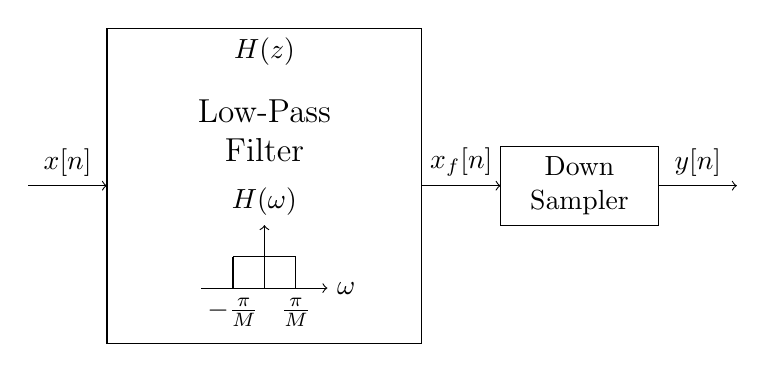
\begin{tikzpicture}

    % Set bounding box dimensions
    \pgfmathsetmacro{\boxsize}{2}
    
    % Draw bounding box
    \draw[black] (-\boxsize,-\boxsize) rectangle (\boxsize,\boxsize);
    
    % Draw arrow and label for x[n]
    \draw[->] (-\boxsize - 1, 0) -- (-\boxsize, 0) node[midway, above] {\(x[n]\)};
    
    % Draw arrow and label for x_f[n], pointing to the downsampler box
    \draw[->] (\boxsize, 0) -- (\boxsize + 1, 0) node[midway, above] {\(x_f[n]\)};
    
    % Draw H(z) text
    \node[align=center] at (0, \boxsize - 0.3) {$H(z)$};
    
    % Draw low-pass filter symbol
    \node[align=center, font=\large] at (0, 0.7) {Low-Pass \\ Filter};
    
    % Draw graph and axes
    \begin{scope}[shift={(0,-\boxsize + 0.7)},scale=0.4]
        % Draw axes
        \draw[->] (-2,0) -- (2,0) node[right] {$\omega$};
        \draw[->] (0,0) -- (0,2) node[above] {$H(\omega)$};
       
        % Draw points
        \node[below] at (-1,0) {$-\frac{\pi}{M}$};
        \node[above] at (-1,1) {};
        \node[above] at (1,1) {};
        \node[below] at (1,0) {$\frac{\pi}{M}$};
        
        % Draw lines connecting the points
        \draw (-1,1) -- (1,1);
        \draw (-1,1) -- (-1,0);
        \draw (1,1) -- (1,0);
        \draw (-1,0) -- (1,0);
    \end{scope}
    
    % Draw Down sampler box and label
    \node[draw, align=center, minimum width=2cm, minimum height=1cm] at (\boxsize + 2, 0) (downsampler) {Down \\ Sampler};
   
    
    % Draw arrow and label for y[n], pointing from the downsampler box
    \draw[->] (downsampler.east) -- (\boxsize + 4, 0) node[midway, above] {\(y[n]\)};
\end{tikzpicture}
\end{center}
\begin{enumerate}
%\begin{itemize}
    \item LPF followed by downsampler is known as a decimator.
    \item The primary role of the LPF is to prevent aliasing, earning it the name anti-aliasing filter.
    \item The cutoff frequency for the LPF is set to \(\pi/M\).
    \item When \(M = 2\), the LPF becomes a Half Band Filter (HBF) with a cutoff frequency of \(\pi/2\).
%\end{itemize}
\end{enumerate}
The Python code below is accompanied by corresponding plots shown in
\begin{center}
    \fcolorbox{black}{white}{\parbox{12.5cm}{/codes/decimation.py}}
\end{center}

\begin{figure}[ht]
  \centering
  \includegraphics[scale=0.5]{./dsp/figs/d_input.png}
  \caption{ Input Signal}
  \label{fig:d_input}
\end{figure}

\begin{figure}[ht]
  \centering
  \includegraphics[scale=0.5]{./dsp/figs/d_l_out.png}
  \caption{Output Signal of Low-Pass Filter}
  \label{fig:d_l_out}
\end{figure}

\begin{figure}[ht]
  \centering
  \includegraphics[scale=0.5]{./dsp/figs/output_decimator.png}
  \caption{ Output Signal of Decimator}
  \label{fig:output_decimator}
\end{figure}
\begin{figure}[ht]
  \centering
  \includegraphics[scale=0.5]{./dsp/figs/output_downsampler.png}
  \caption{Output Signal of Downsampler Without LPF}
  \label{fig:output_downsampler}
\end{figure}
In Figure \ref{fig:d_input}, the input signal composed of multiple sinusoidal components is shown. The output after applying a low-pass filter is depicted in Figure \ref{fig:d_l_out}. The effect of decimation is visible in Figure \ref{fig:output_decimator}, and the outcome of downsampling without a low-pass filter is illustrated in Figure \ref{fig:output_downsampler}.


\subsection{Upsampler (Expander)}
%\begin{itemize}
\begin{enumerate}
    \item \textbf{Time domain relation between input and output:}
    \begin{align*}
    y[n] = \begin{cases}
    x[n/L], & \text{if } n \text{ is a multiple of } L \\
    0, & \text{otherwise}
\end{cases}
       \end{align*}  
    \item \textbf{Frequency domain relation between input and output:}
    \[
    Y(e^{j\omega}) = X(e^{j(\omega/L)}), \quad \text{for } 0 \leq \omega < 2\pi
    \]
%\end{itemize}
\end{enumerate}
\section{Interpolation}
\begin{enumerate}
    \item Upsampler followed by LPF is known as an interpolator.
    \item The job of LPF is to remove the unwanted image of \(X e^{j\omega}\). Hence, it is known as an anti-imaging filter.
    \item Cutoff frequency is \(\frac{\pi}{L}\).
    \item When \(L = 2\), then the LPF is also known as a Half Band Filter (HBF) with a cutoff frequency of \(\frac{\pi}{2}\).
\end{enumerate}
\begin{figure}[htbp]
\centering
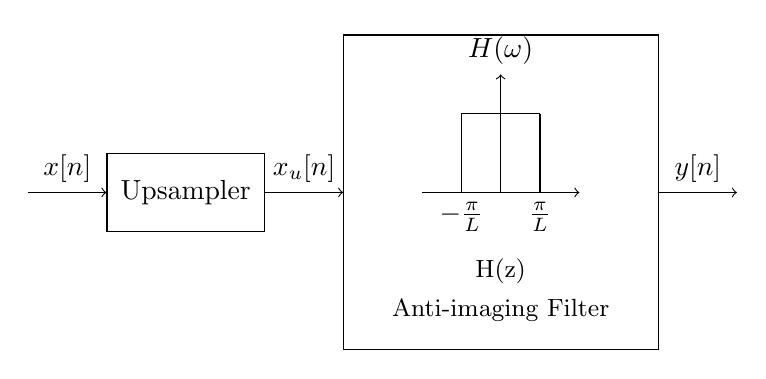
\begin{tikzpicture}
    % Set box dimensions
    \pgfmathsetmacro{\boxwidth}{2}
    \pgfmathsetmacro{\boxheight}{1}
    
  
    % Draw Upsampler box and label
    \node[draw, align=center, minimum width=\boxwidth cm, minimum height=\boxheight cm] at (0, 0) (upsampler) {Upsampler};
    
    \draw[->] (-\boxwidth, 0) -- (upsampler.west) node[midway, above] {\(x[n]\)};
   
    \draw[->] (upsampler) -- node[midway, above] {$x_u[n]$} ++(1*\boxwidth, 0);
    
    % Draw second box for filter and graph
    \node[draw, align=center, minimum width=4cm, minimum height=4cm] at (\boxwidth + 2, 0) (filter) {};
    
  
    \node[align=center, font=\small] at (filter.center |- 0, -1) {H(z)};
     \node[align=center, font=\small] at (filter.center |- 0, -1.5) {Anti-imaging Filter};
    
  
    
    % Draw graph and axes inside the filter box
    \begin{scope}[shift={(filter.center)}]
        % Draw axes
        \draw[->] (-1,0) -- (1,0) node[right] {};
        \draw[->] (0,0) -- (0,1.5) node[above] {$H(\omega)$};
       \iffalse
        % Draw points
        \node[below] at (-0.5,0) {$-\frac{\pi}{L}$};
        \node[above] at (-0.5,1) {};
        \node[above] at (0.5,1) {};
        \node[below] at (0.5,0) {$\frac{\pi}{L}$};
        
        % Draw lines connecting the points
        \draw (-0.5,1) -- (0.5,1);
        \draw (-0.5,1) -- (-0.5,0);
        \draw (0.5,1) -- (0.5,0);
        \draw (-0.5,0) -- (0.5,0);
        \fi
        
        
        
        % Draw points
        \node[below] at (-0.5,0) {$-\frac{\pi}{L}$};
        \node[above] at (-0.5,1) {};
        \node[above] at (0.5,1) {};
        \node[below] at (0.5,0) {$\frac{\pi}{L}$};
        
        % Draw lines connecting the points
        \draw (-0.5,1) -- (0.5,1);
        \draw (-0.5,1) -- (-0.5,0);
        \draw (0.5,1) -- (0.5,0);
        \draw (-0.5,0) -- (0.5,0);
    \end{scope}
    
    % Draw arrow and label for y[n], pointing from filter box
    \draw[->] (filter.east) -- (\boxwidth + 4+ \boxwidth/2, 0) node[midway, above] {\(y[n]\)};
\end{tikzpicture}
\caption{Interpolation and Filtering Diagram}
    \label{fig:interpolation-diagram}
\end{figure}
The Python code demonstrates upsampling and interpolation of a discrete input signal using a half-band filter. It generates plots illustrating the signal processing steps 
and visualizes the magnitude response in the frequency domain.
\begin{center}
    \fcolorbox{black}{white}{\parbox{12.5cm}{/codes/interpolation.py}}
\end{center}

\begin{figure}[ht]
  \centering
  \includegraphics[scale=0.8]{./dsp/figs/istem_plots.png}
  \caption{ Input Signal}
  \label{fig:istem_plots}
\end{figure}
\begin{figure}[ht]
  \centering
  \includegraphics[scale=0.8]{./dsp/figs/interpolated_output.png}
  \caption{Interpolated Output Signal and Frequency Response}
  \label{fig:interpolated_output}
\end{figure}
\begin{figure}[ht]
  \centering
  \includegraphics[scale=0.8]{./dsp/figs/iupsampled_output.png}
  \caption{Upsampled Input Signal and Frequency Response}
  \label{fig:iupsampled_output}
\end{figure}
In the results presented in Figure \ref{fig:istem_plots}, we can observe the original input signal. The interpolated output signal and its corresponding frequency response are illustrated in Figure \ref{fig:interpolated_output}. Similarly, Figure \ref{fig:iupsampled_output} provides insight into the upsampled input signal and its frequency response.

%\end{document}





